% !TeX spellcheck = en_US
% !TeX encoding = utf8
% !TeX program = xelatex
% !BIB program = bibtex
% \documentclass[mathserif,compress,12pt]{ctexbeamer}
\documentclass[12pt,notes,mathserif]{beamer}
% \documentclass[draft]{beamer}	
\usetheme{Singapore}
% \usetheme{Hannover}
%\usepackage{pgfpages}
%\setbeameroption{show notes on second screen}

\usepackage[british]{babel}
\usepackage{graphicx,hyperref,url}
% \usepackage{ru}
\usepackage{mmstyles}

\usepackage{listings,bm}
\usepackage{mathrsfs}
\usefonttheme[onlymath]{serif}
\usepackage{fontspec}
\usepackage{xeCJK}
% \pgfdeclareimage[width=\paperwidth,height=\paperheight]{bg}{background}
% \setbeamertemplate{background}{\pgfuseimage{bg}}
%% columns
\newcommand{\begincols}[1]{\begin{columns}{#1}}
\newcommand{\stopcols}{\end{columns}}
% \usepackage[backend=biber]{biblatex}
% \bibliography{./ref.bib}
%\addbibresource{ref.bib}
\usepackage{indentfirst}
\usepackage{longtable}
\usepackage{float}
%\usepackage{picins}
\usepackage{rotating}
\usepackage{subfigure}
\usepackage{tabu}
\usepackage{amsmath}
\usepackage{amssymb}
\usepackage{setspace}
\usepackage{amsfonts}
\usepackage{appendix}
\usepackage{listings}
\usepackage{xcolor}
\usepackage{colortbl}
\usepackage{geometry}
% \setCJKfamilyfont{cjkhwxk}{SimSun}
% \newcommand*{\cjkhwxk}{\CJKfamily{cjkhwxk}}
%\newfontfamily{\consolas}{Consolas}
%\newfontfamily{\monaco}{Monaco}
%\setmonofont[Mapping={}]{Consolas}	%英文引号之类的正常显示,相当于设置英文字体
%\setsansfont{Consolas} %设置英文字体 Monaco, Consolas,  Fantasque Sans Mono
% \setmainfont{Times New Roman}
% \newfontfamily{\consolas}{Times New Roman}
% \newfontfamily{\monaco}{Arial}
% \setCJKmainfont{Times New Roman}
%\setmainfont{MONACO.TTF}
%\setsansfont{MONACO.TTF}
\newcommand{\verylarge}{\fontsize{60pt}{\baselineskip}\selectfont}  
\newcommand{\chuhao}{\fontsize{44.9pt}{\baselineskip}\selectfont}  
\newcommand{\xiaochu}{\fontsize{38.5pt}{\baselineskip}\selectfont}  
\newcommand{\yihao}{\fontsize{27.8pt}{\baselineskip}\selectfont}  
\newcommand{\xiaoyi}{\fontsize{25.7pt}{\baselineskip}\selectfont}  
\newcommand{\erhao}{\fontsize{23.5pt}{\baselineskip}\selectfont}  
\newcommand{\xiaoerhao}{\fontsize{19.3pt}{\baselineskip}\selectfont} 
\newcommand{\sihao}{\fontsize{14pt}{\baselineskip}\selectfont}      % 字号设置  
\newcommand{\xiaosihao}{\fontsize{12pt}{\baselineskip}\selectfont}  % 字号设置  
\newcommand{\wuhao}{\fontsize{10.5pt}{\baselineskip}\selectfont}    % 字号设置  
\newcommand{\xiaowuhao}{\fontsize{9pt}{\baselineskip}\selectfont}   % 字号设置  
\newcommand{\liuhao}{\fontsize{7.875pt}{\baselineskip}\selectfont}  % 字号设置  
\newcommand{\qihao}{\fontsize{5.25pt}{\baselineskip}\selectfont}    % 字号设置 

\graphicspath{{./fig/}}

% \setbeamertemplate{footnote}{%
%   \hangpara{2em}{1}%
%   \makebox[2em][l]{\insertfootnotemark}\footnotesize\insertfootnotetext\par%
% }

\definecolor{cred}{rgb}{0.6,0,0}
\definecolor{cgreen}{rgb}{0.25,0.5,0.35}
\definecolor{cpurple}{rgb}{0.5,0,0.35}
\definecolor{cdocblue}{rgb}{0.25,0.35,0.75}
\definecolor{cdark}{rgb}{0.95,1.0,1.0}
\lstset{
	language=R,
	numbers=left,
	numberstyle=\tiny\color{black},
	keywordstyle=\color{cpurple}\consolas,
	commentstyle=\color{cgreen}\consolas,
	stringstyle=\color{cred}\consolas,
	frame=single,
	escapeinside=``,
	xleftmargin=1em,
	xrightmargin=1em, 
	backgroundcolor=\color{cdark},
	aboveskip=1em,
	breaklines=true,
	tabsize=3
} 

\providecommand{\tightlist}{%
  \setlength{\itemsep}{0pt}\setlength{\parskip}{0pt}}

  
% The title of the presentation:
%  - first a short version which is visible at the bottom of each slide;
%  - second the full title shown on the title slide;
\title[]{Evaluating models fairly}

% Optional: a subtitle to be dispalyed on the title slide
\subtitle{\Large MLP Tips}

% The author(s) of the presentation:
%  - again first a short version to be displayed at the bottom;
%  - next the full list of authors, which may include contact information;
\author[YingmingLi]{Yingming Li \\ yingming@zju.edu.cn}
% The institute:
%  - to start the name of the university as displayed on the top of each slide
%    this can be adjusted such that you can also create a Dutch version
%  - next the institute information as displayed on the title slide

\institute[DSERC, ZJU]{Data Science \& Engineering Research Center, ZJU}

% Add a date and possibly the name of the event to the slides
%  - again first a short version to be shown at the bottom of each slide
%  - second the full date and event name for the title slide
\date[\today]{\today}

\begin{document}

\AtBeginSection[]
{
	\begin{frame}
		\frametitle{Outline}
		\tableofcontents[currentsection]
	\end{frame}
}

% \AtBeginSubsection[2-]
% {
%    \begin{frame}
%        \frametitle{Outline}
%        \tableofcontents[currentsection]
%    \end{frame}
% }
\begin{frame}[c]
	\titlepage
	\begin{center}
		Adapted from slides provided by Prof.  Michael Mandel.
	\end{center}
\end{frame}

% 2
\begin{frame}[c]
	\frametitle{MLP design parameters}
	\begin{itemize}
		\item  Several parameters to choose when designing an MLP (best to evaluate empirically)
		\item Number of hidden layers
		\item Number of units in each hidden layer
		\item Activation function
		\item Error function
	\end{itemize}
\end{frame}
% 3
\begin{frame}[c]
	\frametitle{Optimization tricks}
	\begin{itemize}
		\item  For a given network, local minima of the cost function are possible
		\item  Many tricks exist to try to find better local minima
		      \begin{itemize}
			      \item Momentum: mix in gradient from step

			      \item Weight initialization: small random values

			      \item  Stopping criterion: early stopping

			      \item Learning rate annealing: start with large, slowly shrink

			      \item Second order methods: use a separate for each parameter or pair of parameters based on local curvature

			      \item Randomization of training example order

			      \item Regularization, i.e., terms in $E(w)$ that only depend on $w$

		      \end{itemize}

	\end{itemize}

\end{frame}
% 4
\begin{frame}[c]
	\frametitle{Learning rate control: momentum}
	\begin{itemize}
		\item To ease oscillating weights due to large $\eta$, some inertia (momentum) of weight update is added
		      \[
			      \Delta w_{ji}(n)=\eta \delta_jy_i+\alpha\Delta w_{ji}(n-1), ~~~0<\alpha<1
		      \]\vspace*{-5mm}
		      \begin{itemize}
			      \item In the downhill situation,$\Delta w_{ji}(n)\approx \frac{\eta}{1-\alpha}\delta_jy_i$
			            \begin{itemize}
				            \item  thus accelerating learning by a factor of $1/(1-\alpha)$

			            \end{itemize}
			      \item In the oscillating situation, it smooths weight change, thus stabilizing oscillations

		      \end{itemize}
	\end{itemize}
\end{frame}
% 5
\begin{frame}[c]
	\frametitle{Input pre-processing}
	\begin{itemize}
		\item Remove mean
		      \begin{itemize}
			      \item  Avoids extra update steps to learn it

		      \end{itemize}
		\item Divide by standard deviation
		      \begin{itemize}
			      \item Or whiten by multiplying by the inverse of square root of the covariance matrix

			      \item Make dimensions commensurate

			      \item Scales curvature of error surface to be less canyon-like

		      \end{itemize}

	\end{itemize}

\end{frame}
% 6
\begin{frame}[c]
	\frametitle{Weight initialization}
	\begin{itemize}
		\item Consider a network with one hidden layer and a single output neuron
		\item What happens if we initialize all weights to 0?
	\end{itemize}
	\begin{center}
		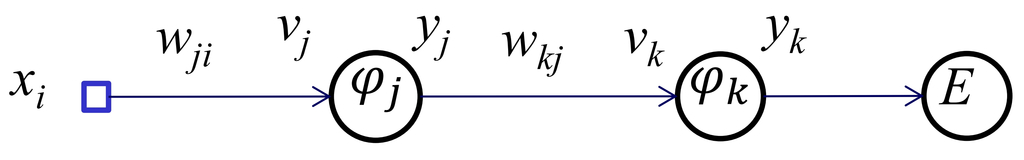
\includegraphics[width=0.47\linewidth]{fig/lec66.jpg}
	\end{center}
	\[
		\begin{array}{c}
			y_k=\varphi_k\left(\sum\nolimits_jw_{kj}\varphi_j\left(\sum\nolimits_iw_{ji}x_i\right)_j\right) \\
			\frac{\partial}{\partial w_{ki}}E(\mathbf{w})=-e_k\varphi'(v_k)y_j                            \\
			\frac{\partial}{\partial w_{ji}}E(\mathbf{w})=-e_j\varphi'(v_j)x_i                            \\
		\end{array}
	\]
\end{frame}
% 7
\begin{frame}[c]
	\frametitle{Weight initialization}
	\begin{itemize}
		\item Break symmetry by initializing with random values
		\item If inputs are normalized, they are uncorrelated, with zero-mean, and unit-variance, and all weights are initialized to 0, 
		\item Then, every neuron in the network computes the same output, and also computes the same gradients during backpropagation and undergoes the exact same parameter updates. The network never converges. 
		\item Break symmetry accelerate convergence.
	\end{itemize}
\end{frame}

% 8
\begin{frame}[c]
	\frametitle{Hyperbolic tangent function}
	\begin{center}
		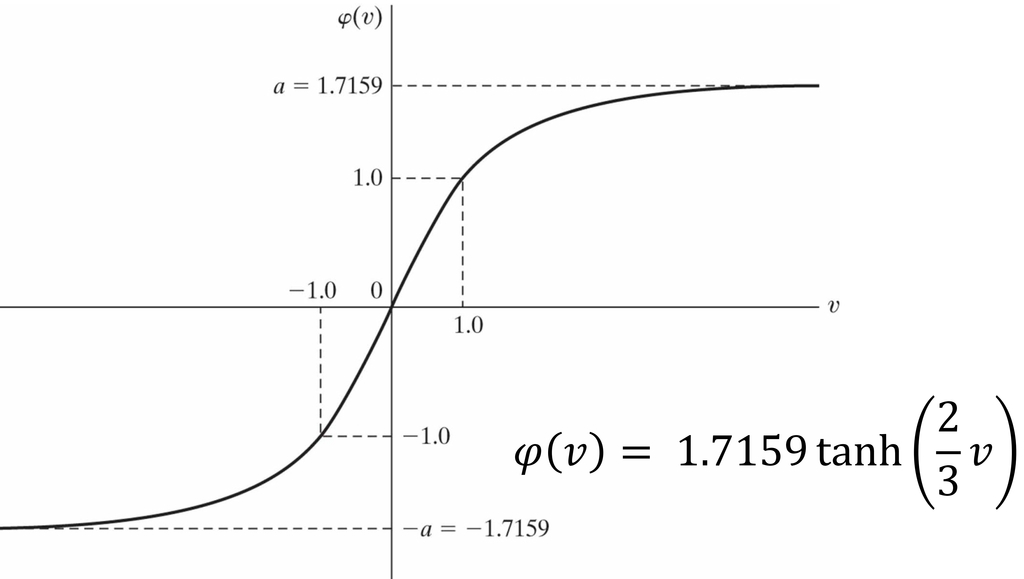
\includegraphics[width=0.95\linewidth]{fig/lec68.jpg}
	\end{center}
\end{frame}

% 9
\begin{frame}[c]
	\frametitle{Hyperbolic tangent function}
	\begin{center}
		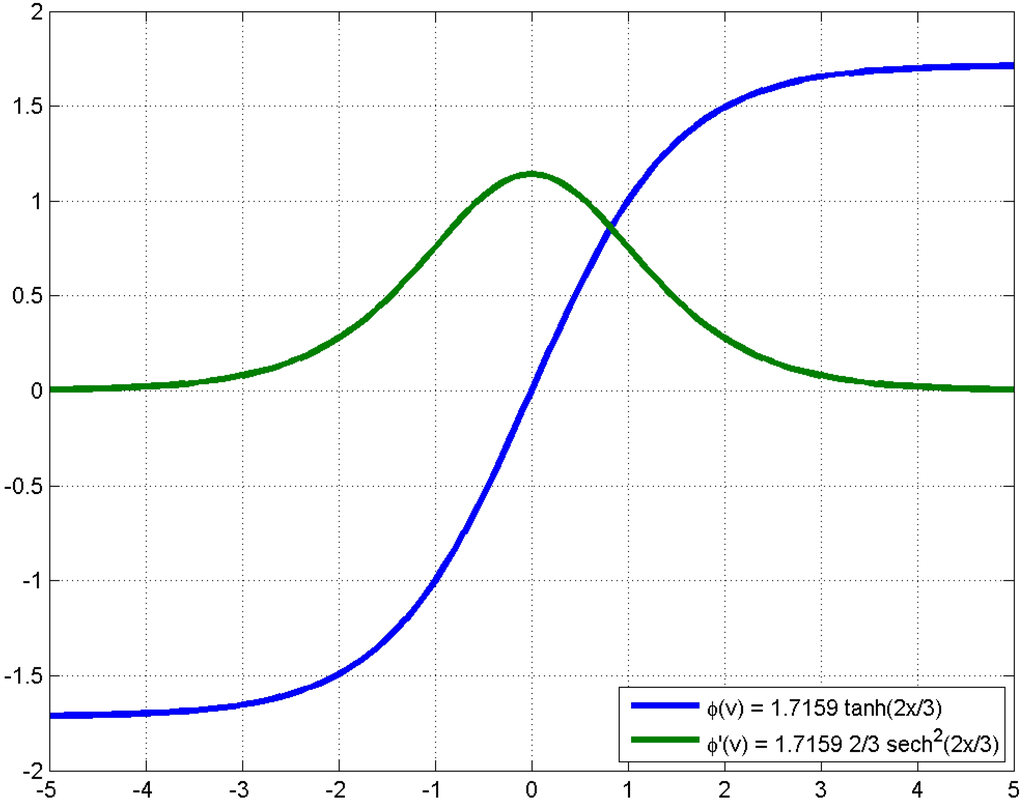
\includegraphics[width=0.7\linewidth]{fig/lec69.jpg}
	\end{center}
\end{frame}

% 10
\begin{frame}[c]
	\frametitle{Weight initialization}
	\[
		\begin{array}{rl}
			\sigma_{y_i}^2 & =E_x\{y_i^2\}=E_x\left\{\varphi^2\left(\sum\limits_jw_{ij}x_j\right)\right\} \\[5mm]
			               & \approx E_x \left\{\left(\sum\limits_jw_{ij}x_j\right)^2\right\}\approx
			\sum\limits_jw_{ij}^2E_x\{x_j^2\}                                                           \\
			               & =\sum\limits_{j=1}^mw_{ij}^2
		\end{array}
	\]
	\begin{itemize}
		\item So in order to make $\sigma_{y_i}^2=1$ 
		      \begin{itemize}
			      \item Initialize $w_{ij}$ randomly with $\sigma_w^2=\frac{1}{m}$
		      \end{itemize}
	\end{itemize}
\end{frame}

% 11
\begin{frame}[c]
	\frametitle{Debugging: Gradient checking}
	\begin{itemize}
		\item Is your backpropagation code working properly?
		      \begin{itemize}
			      \item \ie, is it computing the right gradient?
		      \end{itemize}
		\item Backpropagation computes
		      \[
			      \nabla_{\mathbf{w}}E(\mathbf{x}_p;\mathbf{w})=
			      \left[
				      \frac{\partial E}{\partial \vw_{111}},
				      \frac{\partial E}{\partial \vw_{121}},\cdots,
				      \frac{\partial E}{\partial \vw_{NML}}
				      \right]
		      \]
		      \begin{itemize}
			      \item where $w_{i_1i_2l}$ is the weight in layer $l$ connecting neurons $i_1$ and $i_2$
		      \end{itemize}
		\item 𝑖Compute the gradient {\bf numerically} and compare
	\end{itemize}
\end{frame}

% 12
\begin{frame}[c]
	\frametitle{Recall: Gradient illustration}
	\begin{center}
		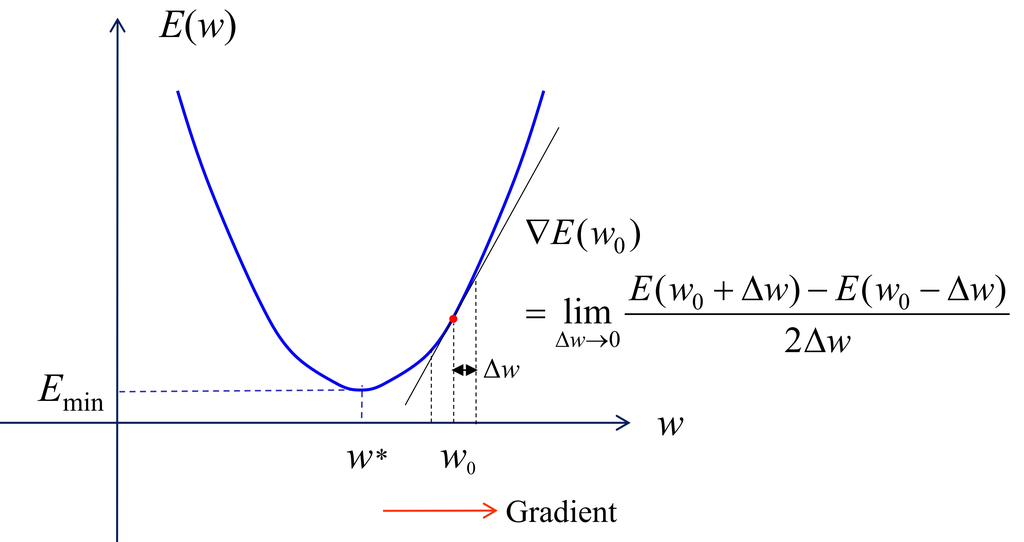
\includegraphics[width=0.99\linewidth]{fig/lec612.jpg}
	\end{center}
\end{frame}

% 13
\begin{frame}[c]
	\frametitle{Debugging: Gradient checking}
	\begin{itemize}
		\item  One-sided numerical gradient:
		      \[
			      \frac{\partial E}{\partial w_{i_1i_2l}}\approx
			      \frac{1}{\delta}
			      \bigg(E\left(\mathbf{x}_p;\mathbf{w}+\delta\mathbf{1}_{i_1i_2l}\right)-E(\mathbf{x}_p;\mathbf{w})\bigg)
		      \]\vspace*{-5mm}
		      \begin{itemize}
			      \item where $\mathbf{1}_{i_1i_2l}$ is a vector that is 1 at entry $1_{i_1i_2l}$ and 0 everywhere else and $\delta$ is a ``small'' constant
		      \end{itemize}
		\item Two-sided numerical gradient:
		      \[
			      \frac{1}{2\delta}\bigg(E\left(\mathbf{x}_p;\mathbf{w}+\delta\mathbf{1}_{i_1i_2l}\right)-E(\mathbf{x}_p;\mathbf{w}-\delta\mathbf{1}_{i_1i_2l})\bigg)
		      \]\vspace*{-5mm}
		      \begin{itemize}
			      \item More accurate approximation
			      \item But requires twice as many evaluations of $E(\mathbf{x}_p;\mathbf{w})$
		      \end{itemize}
	\end{itemize}
\end{frame}

% 14
\begin{frame}[c]
	\frametitle{Debugging: Gradient checking}
	\begin{itemize}
		\item  Complexity of backpropagation
		      \begin{itemize}
			      \item 1 forward pass ($O(1)$ multiply and add per weight)
			      \item 1 backward pass ($O(1)$ multiply and add per weight)
		      \end{itemize}
		\item  Complexity of numerical gradient
		      \begin{itemize}
			      \item One-sided: 1 forward pass \textit{per network weight}
			            \begin{itemize}
				            \item  So $W + 1$ forward passes total
			            \end{itemize}
			      \item Two-sided: 2 forward passes \textit{per network weight}

		      \end{itemize}
		\item  So numerical gradient is good for checking correctness of backpropagation

		      \begin{itemize}
			      \item But very slow to use in training, especially for large $W$
		      \end{itemize}
	\end{itemize}
\end{frame}


% 15
\begin{frame}[c]
	\frametitle{Gradient checking procedure}
	\begin{itemize}
		\item 𝑝Select an example data point, $\mathbf{x}_p$, initialize $\mathbf{w}$
		\item Compute the gradient of $E(\mathbf{x}_p;\mathbf{w})$ using backprop
		      \begin{itemize}
			      \item Gives a vector of derivatives, one for each weight in the network
		      \end{itemize}
		\item Compute the gradient numerically
		      \begin{itemize}
			      \item Evaluate $E(\mathbf{x}_p;\mathbf{w})$
			      \item Loop over each weight in the network
			            \begin{itemize}
				            \item Evaluate $E(\mathbf{x}_p;\mathbf{w}+\delta \mathbf{1}_{i_1i_2l})$, compute partial derivative
			            \end{itemize}
		      \end{itemize}
		\item If they are not the same, look for patterns as a
		      function of $i_1i_2l$, etc
	\end{itemize}
\end{frame}

% 16
\begin{frame}[c]
	\frametitle{How to select $\delta$?}
	\begin{itemize}
		\item 𝛿$\delta$ too big means derivative might be different at $E(\mathbf{x}_p;\mathbf{w}+\delta \mathbf{1}_{i_1i_2l})$ and $E(\mathbf{x}_p;\mathbf{w})$
		      \begin{itemize}
			      \item Leading to a bad estimate using the above formulas
		      \end{itemize}
		\item $\delta$ too small runs into numerical issues
		      \begin{itemize}
			      \item Need to be aware of limitations of floating point math
			      \item For $\delta$ too small, $1+\delta =1$
			      \item This might be around 1e-16, depending on the data type (e.g., float, double)
			      \item So $\delta= 1$e-8 might be reasonable
		      \end{itemize}
	\end{itemize}
\end{frame}

% 17
\begin{frame}[c]
	\frametitle{How to select $\delta$?}
	\begin{center}
		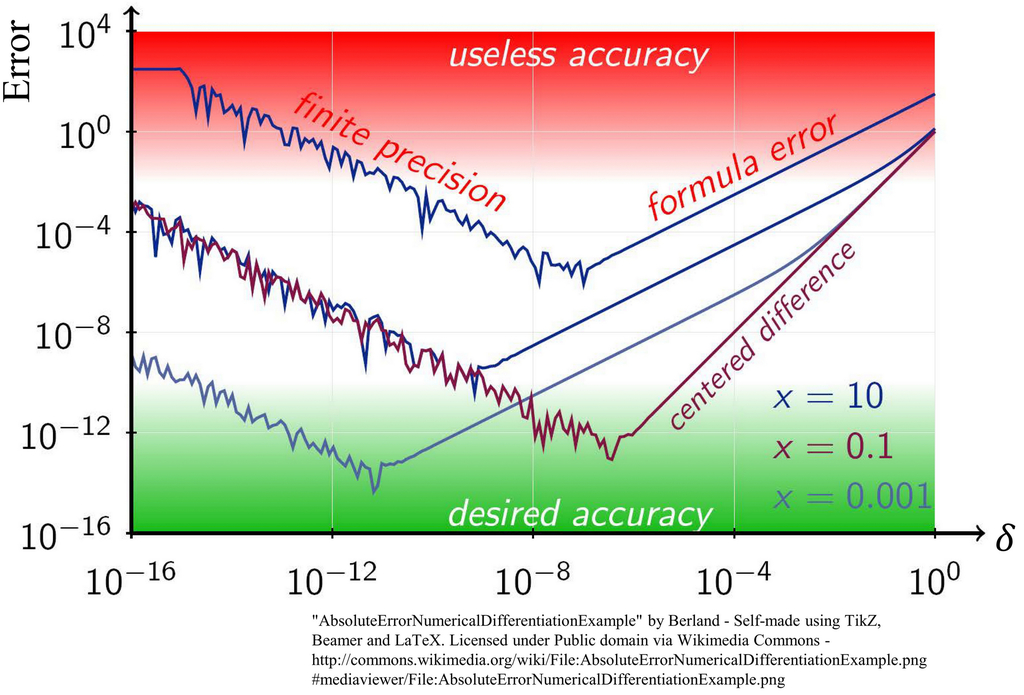
\includegraphics[width=0.99\textwidth]{fig/lec617.jpg}
	\end{center}
\end{frame}









\begin{frame}
	\begin{center}
		\chuhao Thank you! %\fontspec{LHANDW.TTF}
	\end{center}
\end{frame}
\end{document}
